% Digital Logic Report Template
% Created: 2020-01-10, John Miller

%==========================================================
%=========== Document Setup  ==============================

% Formatting defined by class file
\documentclass[11pt]{article}

% ---- Document formatting ----
\usepackage[margin=1in]{geometry}	% Narrower margins
\usepackage{booktabs}				% Nice formatting of tables
\usepackage{graphicx}				% Ability to include graphics

%\setlength\parindent{0pt}	% Do not indent first line of paragraphs 
\usepackage[parfill]{parskip}		% Line space b/w paragraphs
%	parfill option prevents last line of pgrph from being fully justified

% Parskip package adds too much space around titles, fix with this
\RequirePackage{titlesec}
\titlespacing\section{0pt}{8pt plus 4pt minus 2pt}{3pt plus 2pt minus 2pt}
\titlespacing\subsection{0pt}{4pt plus 4pt minus 2pt}{-2pt plus 2pt minus 2pt}
\titlespacing\subsubsection{0pt}{2pt plus 4pt minus 2pt}{-6pt plus 2pt minus 2pt}

% ---- Hyperlinks ----
\usepackage[colorlinks=true,urlcolor=blue]{hyperref}	% For URL's. Automatically links internal references.

% ---- Code listings ----
\usepackage{listings} 					% Nice code layout and inclusion
\usepackage[usenames,dvipsnames]{xcolor}	% Colors (needs to be defined before using colors)

% Define custom colors for listings
\definecolor{listinggray}{gray}{0.98}		% Listings background color
\definecolor{rulegray}{gray}{0.7}			% Listings rule/frame color

% Style for Verilog
\lstdefinestyle{Verilog}{
	language=Verilog,					% Verilog
	backgroundcolor=\color{listinggray},	% light gray background
	rulecolor=\color{blue}, 			% blue frame lines
	frame=tb,							% lines above & below
	linewidth=\columnwidth, 			% set line width
	basicstyle=\small\ttfamily,	% basic font style that is used for the code	
	breaklines=true, 					% allow breaking across columns/pages
	tabsize=3,							% set tab size
	commentstyle=\color{gray},	% comments in italic 
	stringstyle=\upshape,				% strings are printed in normal font
	showspaces=false,					% don't underscore spaces
}

% How to use: \Verilog[listing_options]{file}
\newcommand{\Verilog}[2][]{%
	\lstinputlisting[style=Verilog,#1]{#2}
}




%======================================================
%=========== Body  ====================================
\begin{document}

\title{ELC 2137 Lab 5: Intro to Verilog}
\author{Celaine Hornsby}

\maketitle


\section*{Summary}
In this lab we learned how to code the circuits that we built in previous labs. We were able to code the half adder, full adder, and 2-bit adder subtractor that we built in lab. We gained a better understanding of how Verilog and Vivado works from this lab. through the use of design files and simulation files that acted as a test bench for our design files.  


\section*{Q\&A}

\begin{enumerate}
\item What is one thing that you still don't understand about Verilog?\\
	I don't understand how to run simulations of design files. Mine constantly have confusing errors that make my simulations not be able to run. 
\end{enumerate}

\section*{Code}

\Verilog[caption = halfadder.sv]{/Users/Celaine_Hornsby1/Documents/GitHub/Lab05/Lab05/Lab05.srcs/sources_1/new/halfadder.sv}

\Verilog[caption = halfadder test.sv]{/Users/Celaine_Hornsby1/Documents/GitHub/Lab05/Lab05/Lab05.srcs/sim_1/new/halfadder_test.sv}

\Verilog[caption = fulladder.sv]{/Users/Celaine_Hornsby1/Documents/GitHub/Lab05/Lab05/Lab05.srcs/sources_1/new/fulladder.sv}

\Verilog[caption = full adder test.sv]{/Users/Celaine_Hornsby1/Documents/GitHub/Lab05/Lab05/Lab05.srcs/sim_2/new/FA_test.sv}

\Verilog[caption = 2bit]{/Users/Celaine_Hornsby1/Documents/GitHub/Lab05/Lab05/Lab05.srcs/sources_1/new/addsub3.sv}

\Verilog[caption = 2bit test]{/Users/Celaine_Hornsby1/Documents/GitHub/Lab05/Lab05/Lab05.srcs/sim_3/new/as_test.sv}

\section*{Results}
The simulations do match the expected output values. 

\begin{figure}[ht]\centering
	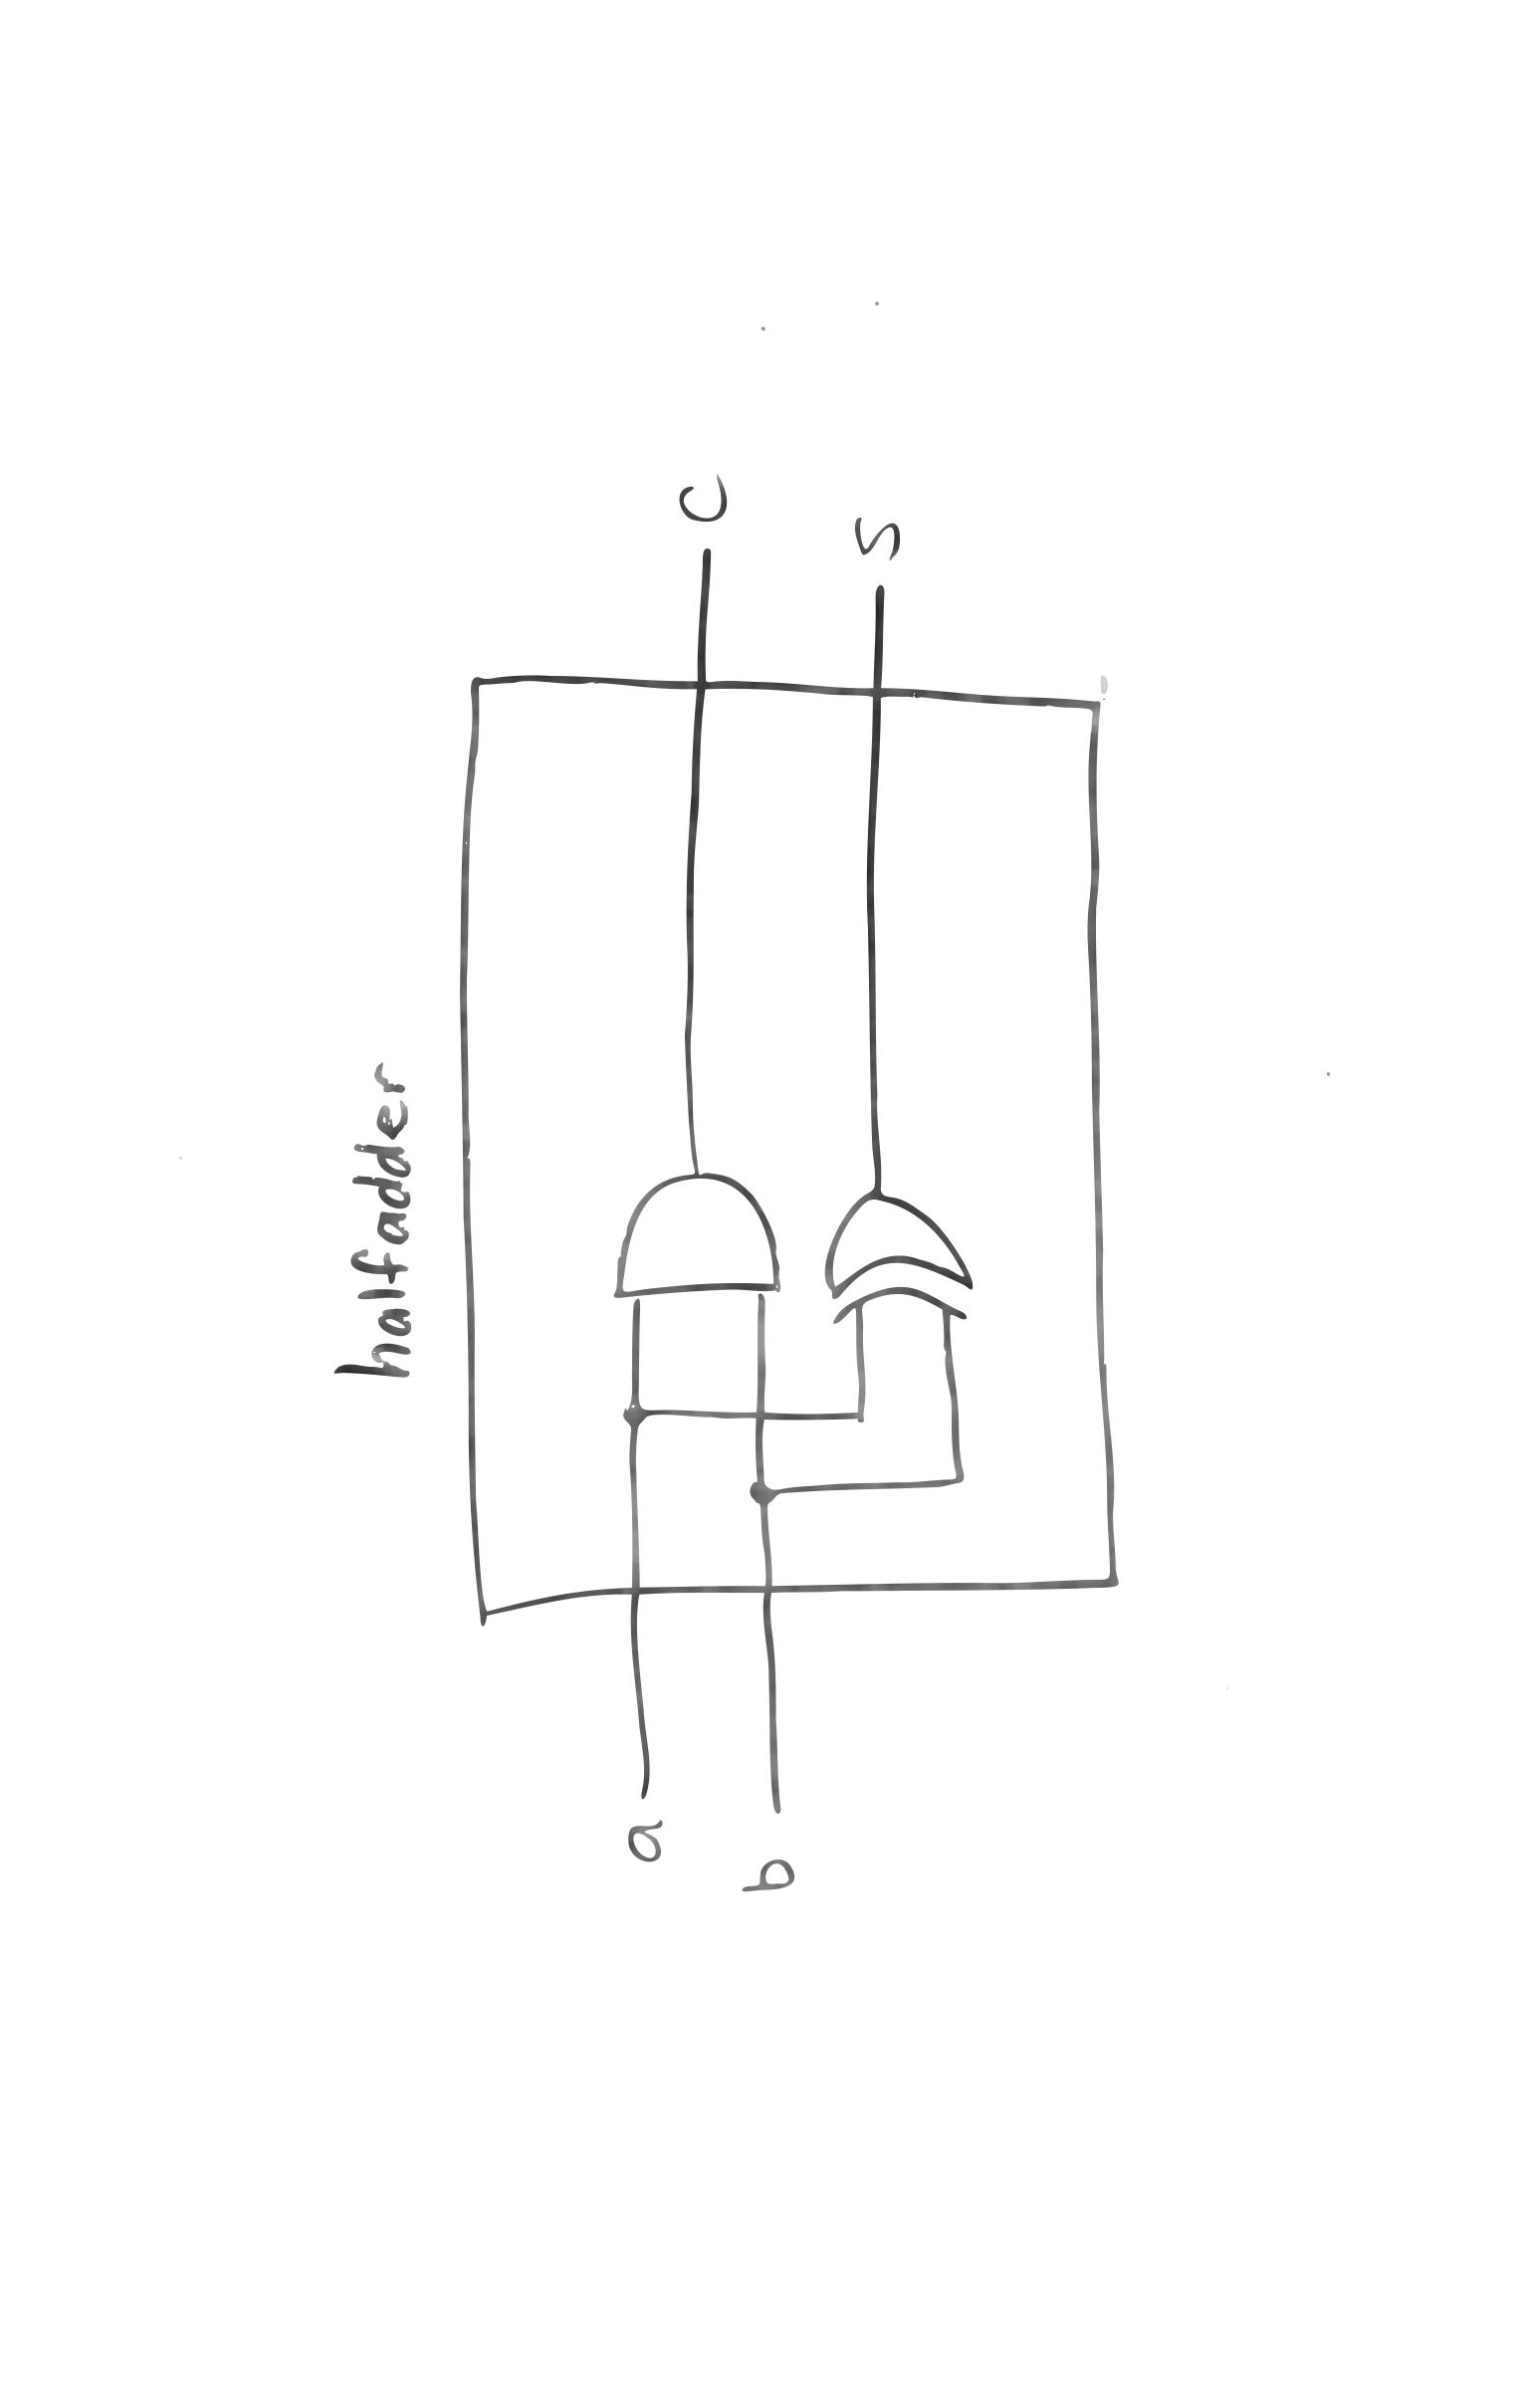
\includegraphics[width=0.6\textwidth]{HA_block}
	\caption{Half Adder Block Diagram}
	\label{fig:ha_block}
\end{figure}

\medskip

\begin{figure}[ht]\centering
	\begin{tabular}{l|rrrr}
		Time (ns): & 0 & 10 & 20 & 30 \\
		\midrule
		a & 0 & 1 & 0 & 1 \\
		b & 0 & 0 & 1 & 1 \\
		\midrule
		c & 0 & 0 & 0 & 1 \\
		s & 0 & 1 & 1 & 0 \\
		\bottomrule
	\end{tabular}\medskip
	
	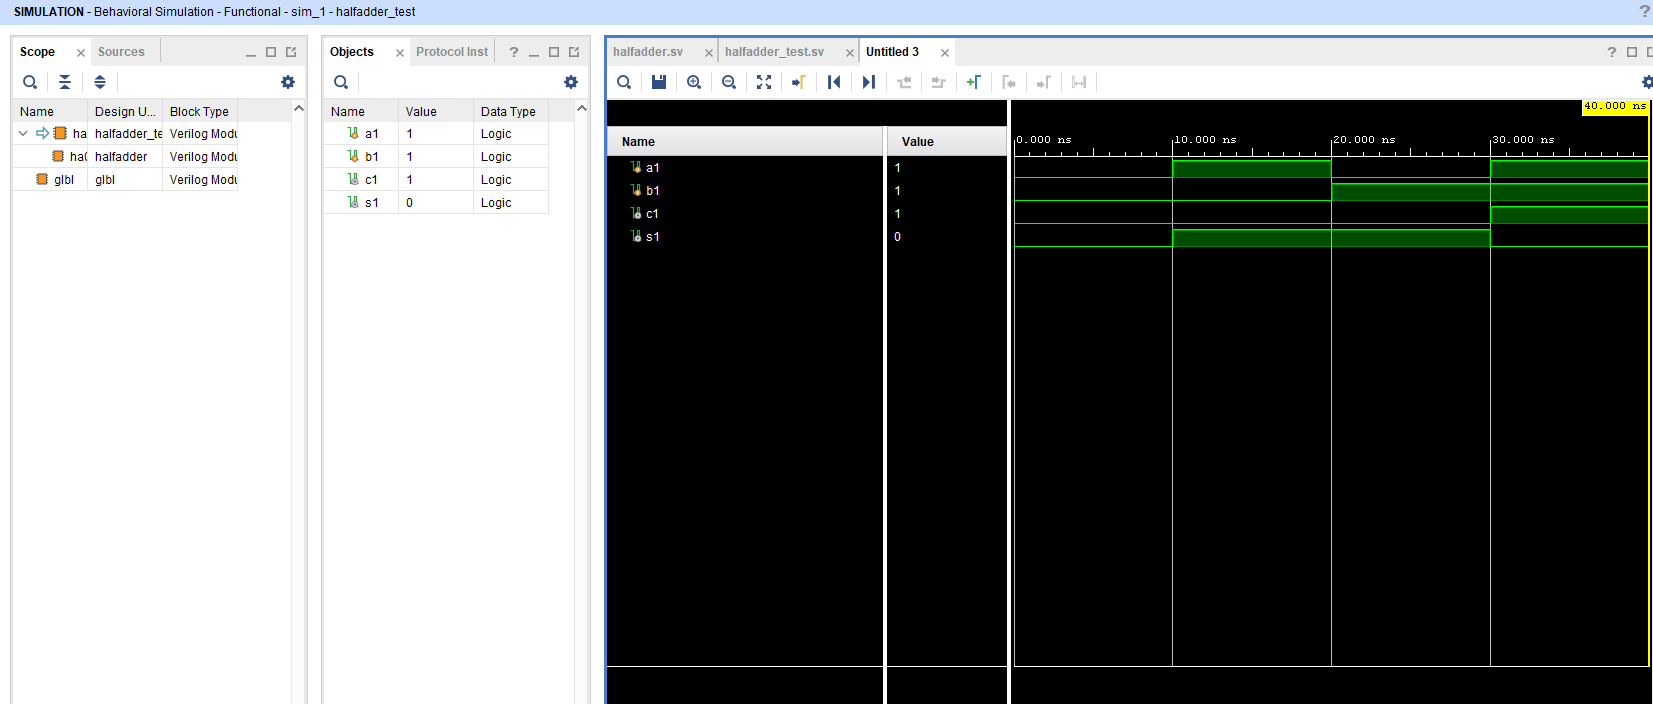
\includegraphics[width=0.9\textwidth,trim = 8.5cm 11.75cm 0cm 2.5cm,clip]{HA_snip}
	\caption{Half Adder waveform and ERT}
	\label{fig:ha_ert}
\end{figure}

\medskip
\medskip

\begin{figure}
	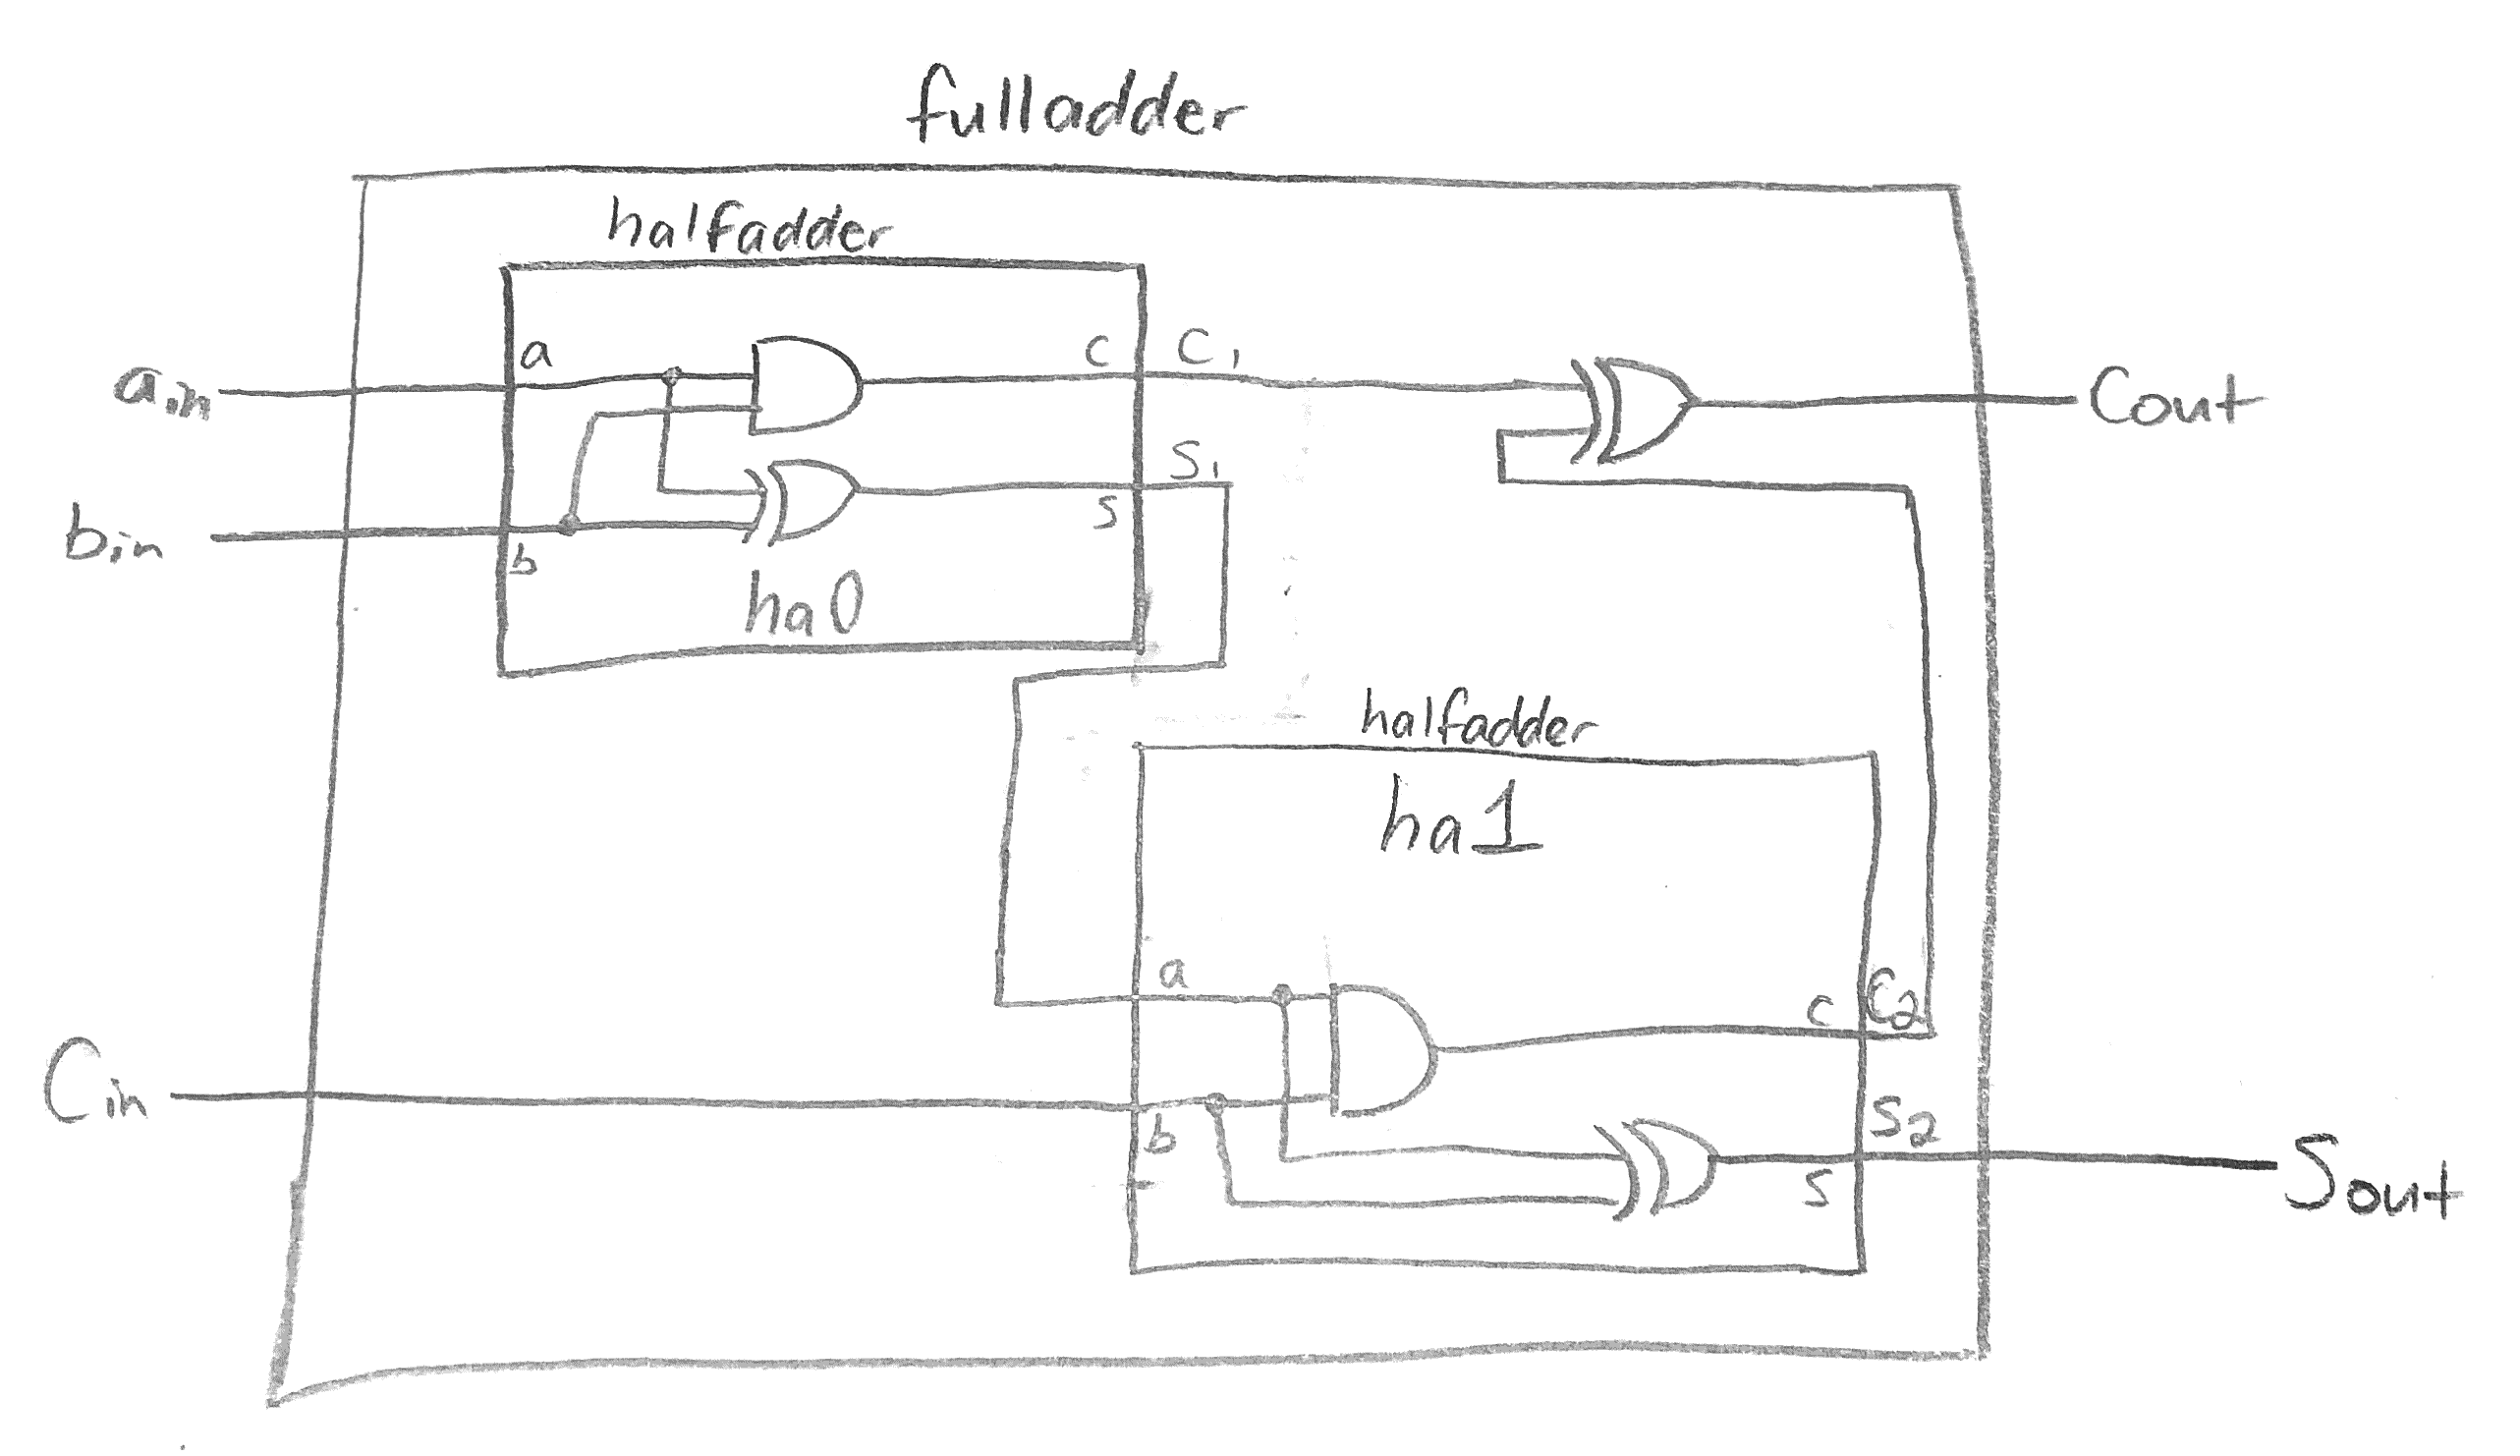
\includegraphics[width=0.9\textwidth]{FA_block}
	\caption{Full Adder Block Diagram}
	\label{fig:fa_block}
\end{figure}
\medskip

\begin{figure}[ht]\centering
	\begin{tabular}{l|rrrrrrrr}
		Time (ns): & 0 & 10 & 20 & 30 & 40 & 50 & 60 & 70\\
		\midrule
		a & 0 & 1 & 0 & 1 & 0 & 1 & 0 & 1\\
		b & 0 & 0 & 1 & 1 & 0 & 0 & 1 & 1\\
		cin & 0 & 0 & 0 & 0 & 1 & 1 & 1 & 1\\ 
		\midrule
		cout & 0 & 0 & 0 & 1 & 0 & 1 & 1 & 1 \\
		sout & 0 & 1 & 1 & 0 & 1 & 0 & 0 & 1\\
		\bottomrule
	\end{tabular}\medskip
	
	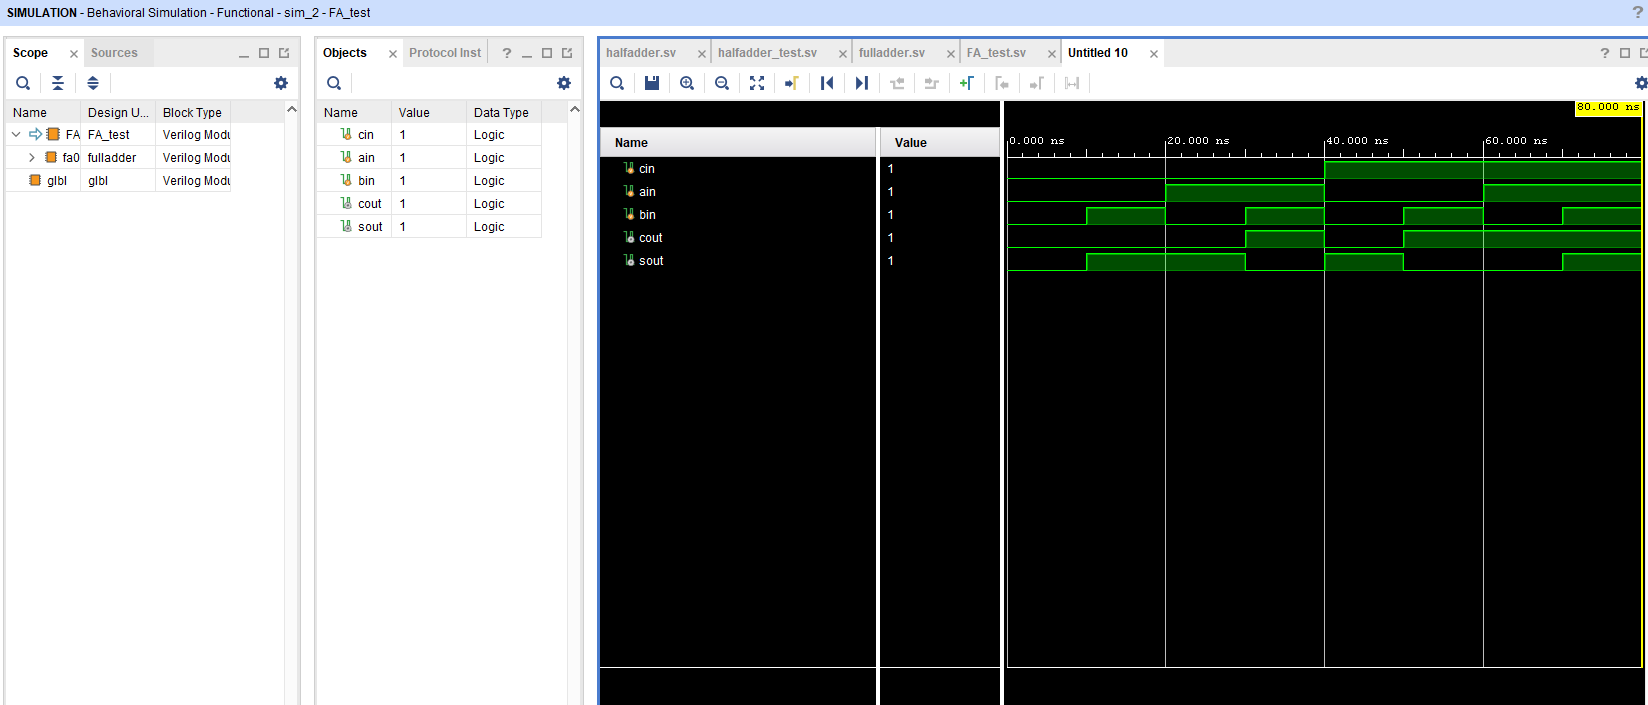
\includegraphics[width=0.9\textwidth,trim = 8.5cm 11cm 0cm 2.5cm,clip]{FA_snip}
	\caption{Full Adder Waveform and ERT}
	\label{fig:fa_ert}
\end{figure}

\medskip
\medskip

\begin{figure}
	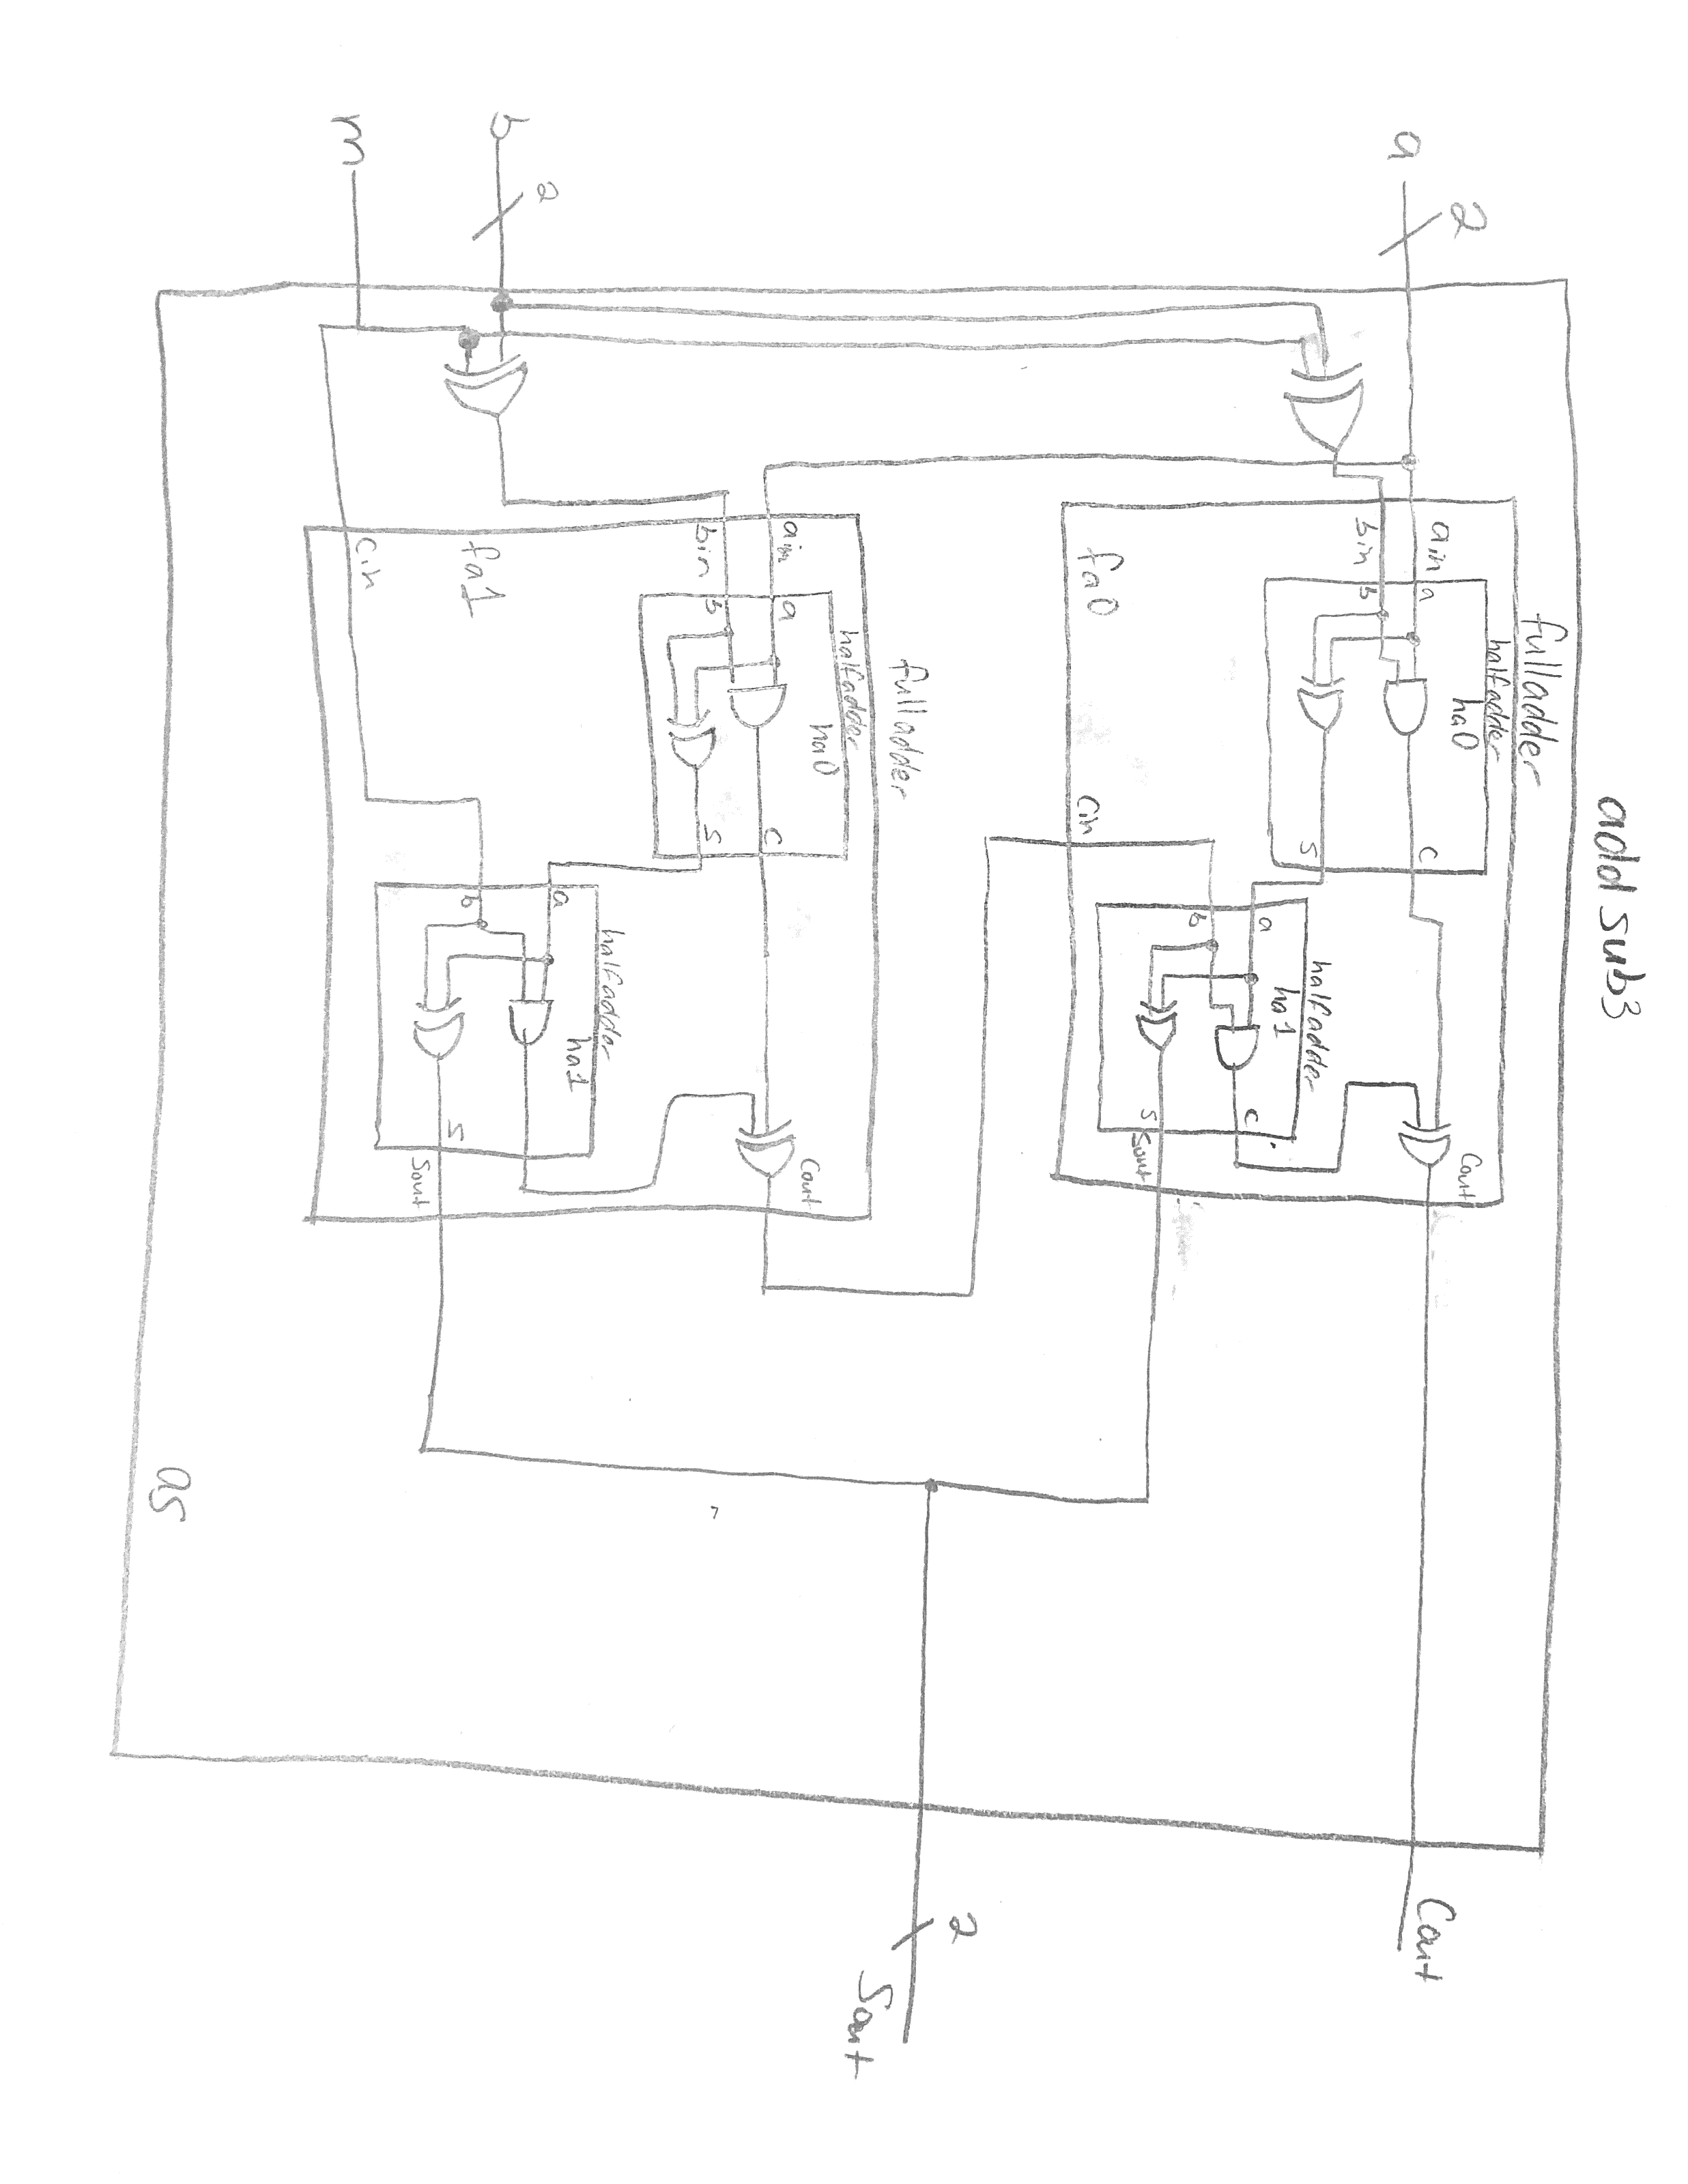
\includegraphics[width=0.9\textwidth]{2B_block}
	\caption{2Bit Adder/Subtractor Block Diagram}
	\label{fig:2B_block}
\end{figure}
\medskip
\begin{figure}[ht]\centering
\begin{tabular}{l|rrrrrrrrrrrr}
	Time (ns): & 0 & 10 & 20 & 30 & 40 & 50 & 60 & 70 & 80 & 90 & 100 & 110\\
	\midrule
	a1  & 0 & 0 & 0 & 1 & 0 & 0 & 0 & 0 & 0 & 1 & 0 & 0\\
	b1  & 1 & 0 & 1 & 1 & 1 & 0 & 1 & 0 & 1 & 1 & 1 & 0\\
	a2  & 0 & 0 & 0 & 0 & 1 & 1 & 0 & 0 & 0 & 0 & 1 & 1\\
	b2  & 0 & 1 & 1 & 0 & 0 & 0 & 1 & 1 & 0 & 0 & 0 & 0\\
	mode & 0 & 0 & 0 & 0 & 0 & 0 & 1 & 1 & 1 & 1 & 1 & 1 \\
	\midrule
	c & 0 & 0 & 0 & 0 & 0 & 0 & 1 & 1 & 1 & 0 & 0 & 0\\
	s1 & 0 & 1 & 1 & 1 & 1 & 1 & 1 & 1 & 0 & 0 & 0 & 1\\
	s2 & 1 & 0 & 1 & 0 & 1 & 0 & 1 & 0 & 1 & 0 & 1 & 0\\
	\bottomrule
\end{tabular}\medskip



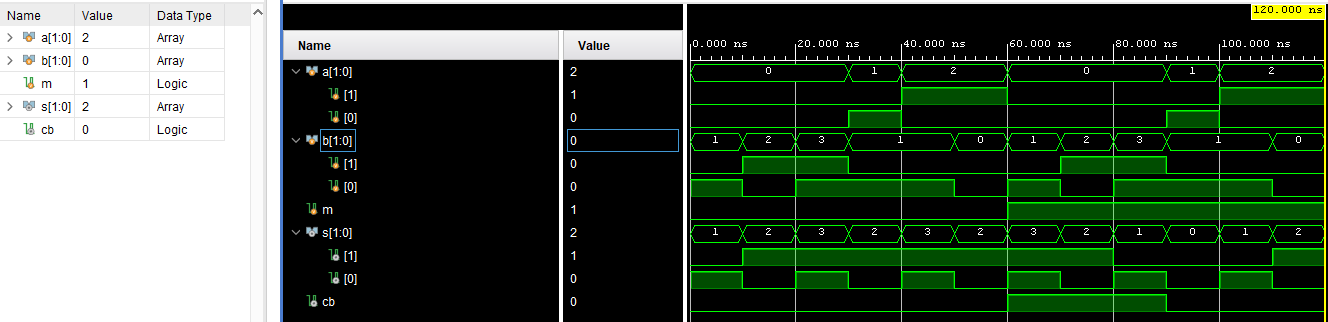
\includegraphics[width=0.9\textwidth]{2B_snip}
\caption{2Bit Adder SubtractorWaveform and ERT}
\label{fig:2B_ert}
\end{figure}

\medskip
\medskip
\end{document}

	

